%\cs{If space allows, I would also put an example image+annotation for RefCOCO and Flickr30kE}
%\gbt{Space doesn't seem to allow :)}
We identified three previously existing resources that can be of use for analysis and modeling of object naming: RefCOCO (and a variant, RefCOCO+), Flickr30k Entities, and Visual Genome. %
Table~\ref{tab:compare} summarizes their main characteristics and compares them to our dataset (last two columns; see Section~\ref{sec:data}).
As the table shows, previous datasets provide between one and three annotations per object, which, we believe, is not enough to assess naming behavior for individual objects and which
motivates our data collection. %, in which we collect 36 names per object.
In the following, we will look at their characteristics in more detail and work out requirements for a dataset that is suitable for a large-scale study of object naming.

\subsection{\refcoco and \refcocop}

Both \refcoco and \refcocop \cite{Yu2016} use the \referit\cite{Kazemzadeh2014} game for collecting referring expressions (RE) for natural objects in real-world images, and are built on top of MS COCO \cite{mscoco}, 
a dataset of images of natural scenes of $91$~common object categories (e.g.,~\cat{dog, pizza, chair}). 
The REs were collected via crowdsourcing in a two-player reference game designed to obtain REs uniquely referring to the target object. 
Specifically, a director and a matcher are presented with an image, and the director produces a RE for an outlined target object. 
The matcher must click on the object she thinks the RE refers to. % (For more details on the datasets see \cite{Yu2016}). 
REs in \refcoco/+ were collected under the constraints that (i) all images contain at least two objects of the same category (80 COCO categories), which results in longer and more complex REs than just the object name, and (ii) in \refcocop the players cannot use location words, urging them to refer to the appearance of objects.
 % \gbt{How come the naming vocabulary size is so large if RefCOCO contains only 80 categories? How did you compute these numbers, are they for names, or whole REs?} \sz{well, 80 categories doesn't mean much as the categories can be very general (like "human") ... and it nicely shows that natural names are much more variable than strict categories}
% Another critical property of the data is that, (iii), not all objects in an image were annotated with REs, may it due to the frequency constraint~(i), or due to the object not being part of the 80 COCO categories.

Table~\ref{tab:compare} shows that the multiple annotations ($2.8$~on average) actually contain a considerable amount of variation in naming (almost~$2$ different names on average per object). 
%However, the small number of annotations per object does not allow for a reliable assessment of speaker agreement. 
However, the small number of annotations per object does not allow to reliably infer object-specific naming preferences or assess speaker agreement. \cs{double-check formulation}

RefCOCO has been used to model and examine the effect of context on referring expression generation in general \cite{Yu2016}, though this work did not look at object names specifically. 
A controlled analysis of the effect of context on choice in naming, as for instance in \cite{graf2016animal}, would require substantial further data annotation as not all objects of an image are annotated with REs and corresponding categories. Hence, so-called distractor objects  \cite{krahmer:2012} and their names cannot be analyzed systematically.
Also, while in \refcoco the elicited names can be assumed to be natural, it is unclear how the additional constraints in \refcocop impact on the naturalness of object naming.
Finally, the underlying set of MS COCO categories is quite small ($80$~categories).
To sum up, \refcoco is suitable for generally modeling referring expressions in context for a restricted set of categories, but less appropriate for analyzing object naming at a large scale.

% \begin{itemize}
% \item[(1)] \textbf{Specific categories}: not available, the $80$~COCO categories tend to be entry-level categories and are not linked to the ImageNet taxonomy (e.g.,~\cat{bird, person, car, bus})
% \item[(2)] \textbf{Exhaustive annotations}: not available, as not all objects were annotated with REs and corresponding categories
% \item[(3)] \textbf{Natural names}: available, though it is unclear how the additional constraints in RefCoco+ impact on the naturalness of object naming
% \end{itemize}

% gbt: I'm commenting out this analysis because it is not really relevant for assessing how useful RefCOCO is to study object naming: what it shows is that names appear at many different levels of a taxonomy, although they tend to be concentrated in middle levels (especially 6-7; in agreement with basic level hypothesis). To me, this is a data result, not a dataset result (clear?). 
% \paragraph{Analysis} We parse REs in \refcoco with the Stanford Dependency Parser and extract the nominal heads. We map these names to their most frequent sense/synset in WordNet.
% We hypothesize that the distance of a name's synset to the root node (\cat{entity}) relates to its specificity.
% We estimate this distance as the minimal path length of all synsets of a word  to the root node.
% Table~\ref{tab:specnames} shows the estimated levels of specificity for object names in the \refcoco data set.
% We observe distances to the root between 2 and 17, meaning that there is a much more fine-grained distinction of levels than the three-way classification adopted in \cite{graf2016animal}.
% Unfortunately, the levels of specificity predicted by WordNet do not seem to reflect linguistic intuitions, e.g.\ \refexp{elephant} is predicted to be more specific than \refexp{panda}.
% At the same time, this overview clearly suggests that object names in \refcoco do not only comprise entry-level categories, but also very general (\refexp{thing}) and very specific names (\refexp{ox}).

% \begin{table*}
% \centering
% \setlength{\tabcolsep}{2pt}
% \begin{small}
% \begin{tabular}{rrl|rrl}
% \toprule
%  spec. &  rel.freq. &                          top 5 names & spec. &  rel.freq. &                          top 5 names \\
% \midrule
%            2 &   $<$ 0.01 &       \tiny                  thing,things & 10 &   0.05 &   elephant,couch,truck,vase,suitcase \\
%            3 &   $<$ 0.01 &    object,group,set,substance,objects & 11 &   $<$ 0.01 &    motorcycle,clock,mom,dad,scissors \\
%            4 &   0.14 &           man,person,piece,head,part & 12 &   $<$ 0.01 &  oven,airplane,suv,taxi,refrigerator  \\
%            5 &   0.10 &       player,glass,baby,front,corner & 13 &   $<$ 0.01 &    laptop,fridge,canoe,orioles,pigeon \\
%            6 &   0.21 &              woman,girl,kid,boy,bowl & 14 &   $<$ 0.01 &   panda,freezer,penguin,rooster,rhino \\
%            7 &   0.25 &            guy,right,chair,lady,bear & 15 &   0.03 &    zebra,giraffe,zebras,giraffes,deer \\
%            8 &   0.11 &           horse,bus,cow,pizza,batter & 16 &  $ <$ 0.01 &       bison,mooses,orang,elks,sambar \\
%            9 &   0.09 &         shirt,car,bike,donut,catcher & 17 &   $<$ 0.01 &           ox,cattle,gnu,mustang,orca \\          
% \bottomrule
% \end{tabular}\caption{Levels of specificity for naming choices in RefCOCO: for each level (distance between name and WordNet root), relative frequency and 5 most frequent names are shown}
% \label{tab:specnames}
% \end{small}
% \label{tab:specnames}
% \end{table*}

\subsection{\flickr}

The \flickr dataset \cite{plummer2015flickr30kentities}
% \footnote{Available at  \url{web.engr.illinois.edu/~bplumme2/Flickr30kEntities}}
augments Flickr30k, a dataset of 30k~images and five sentence-level captions for each of the images, with region-level descriptions extracted from the captions.
Specifically, mentions of the same entities across the five captions of an image are linked to the bounding boxes of the objects they refer to.
% The dataset was designed to advance image description generation and phrase localization in particular \cite{rohrbach2016grounding,plummer2017phrase,yeh2018unsupervised}.

This dataset has three main differences with respect to \refcoco/+: (i) the entity mentions were obtained via an image description task (captioning), as opposed to a referential task; (ii) the images and the production of entity mentions were not subject to any constraints; (iii) a much wider range of categories are covered (cf.\ the number of objects and the vocabulary size in Table~\ref{tab:compare}). %\gbt{Any idea what kind of categories are covered in \flickr?}
Moreover, although no exhaustive annotations of the images are available, the dataset does contain information for the most salient objects in the image, as they are typically mentioned in the captions.
The number of annotations per object, $2.3$\ annotations, is comparable to \refcoco.
This dataset is suitable to analyze object naming in descriptions, for a quite large set of categories (although, again, not enough annotations are available to analyze image-specific naming data).

% \begin{itemize}
% \item[(1)] \textbf{Specific categories}: are not available, object categories tend to be even less specific than those of COCO (e.g.,~\cat{people, animals, bodyparts, clothing}), or are abstract (\cat{other, scene})
% \item[(2)] \textbf{Exhaustive annotations}: are not available
% \item[(3)] \textbf{Natural names}: are available, though object names might not be fully discriminative (as in REs; e.g.,~both animals in the right-most image in Fig.~\ref{fig:graf_genome} are named \refexp{dog})
% \end{itemize}

\subsection{Visual Genome}
\label{sec:vg-survey}

\vgenome (VG, \newcite{krishna2016visualgenome}) is one of the most densely and richly annotated resources currently available in L\&V; here, we focus on aspects immediately relevant to object naming.
%In the following, we will focus on describing aspects immediately relevant to object naming only, but many other annotations are available as well (e.g. questions, paragraphs, etc.)
%\paragraph{Collection and annotation procedure}
\vg aims at providing a full set of descriptions of the scenes which images depict in order to spur complete scene understanding. 
The data collection followed a complex procedure, involving many different rounds of annotation.
The first round of the procedure, and the basic backbone for the further rounds, is a collection of region-based descriptions: workers were asked to describe regions in the image and draw boxes around the corresponding area in the image (for examples, see Figure~\ref{fig:bird}).

In a second, independent round (involving new workers), annotators were asked to process the region descriptions by (i) marking the object names contained in the region description, and (ii) drawing a tight box around the corresponding region. As different region descriptions can potentially mention the same objects, each worker was shown a list of previously marked objects and encouraged to select an existing object rather than annotating a new one.


Some of the main advantages of \vg are its size, with $3.8$~million objects ($108$K images) as opposed to $50$K and $243$K for the other two datasets, and its category coverage, with a vocabulary of object names of $105$K compared to $5$K/$10$K.
Another plus is the fact that it in principle provides exhaustive annotations of objects in an image, often with several region descriptions and possibly object names per object.
This should make it easier to identify factors intervening in naming choices, and to model contextual aspects that may affect them, than in the case of \refcoco.

However, there is a crucial pitfall: As Figure~\ref{fig:bird} shows, there is only a partial linking of objects that are mentioned across different region descriptions; for instance, the first, second, and fifth object IDs in the figure actually correspond to the same object.
Moreover, the regions for the beak of the object (third and fourth object IDs) overlap with those of the bird. 
%This means that the identity of objects cannot be established based on the annotation, which severely limits the usefulness of the data to analyze naming.
%For instance, even though there is a different name (\word{vulture}) for \word{bird} in Figure~\ref{fig:bird}, the annotation suggests that \word{bird} is the only available name. 
Finally, even though there is a different name (\word{vulture}) for \word{bird} in Figure~\ref{fig:bird}, the annotation suggests that \word{bird} is the only available name. 
Hence, the identity of objects cannot be established based on the annotation, which severely limits the usefulness of the data to analyze naming.
The relatively low number of $1.7$~annotations per objects on average in VG (Table~\ref{tab:compare}) and the very small number of objects that have more than one name associated with it ($2$\%) seem to be an effect of this partial linking problem.
We experimented with filtering and merging bounding boxes based on overlap, but this would introduce substantial noise into the data (e.g.,~truly overlapping objects).

Table~\ref{tab:compare} also shows the statistics for the subset of those VG objects that we selected for ManyNames and, here, we find a considerably higher average of $7$~annotations per object. 
We think that this might be an effect of our category selection procedure explained in Section~\ref{sec:data}. However, interestingly, the portion of objects that have different names associated with them is still extremely small.
Note that in contrast, even though RefCOCO has much less annotations per object, there are many objects with different names ($70$\%).


%\cs{The explanation of intervening factors in object naming in the background may be a bit more detailed, such as to really understand the drawbacks of the existing datasets with respect to distractors.}

\subsection{Discussion}

While some existing resources do provide naming data for objects in context, they do not provide \textit{enough} data to systematically assess how variable or stable object naming really is. The RefCOCO data (and to some extent the Flickr30k data) suggests that for most objects there is more than one available name, but it is unclear which name most speakers would prefer or whether there is such a preferred name at all. 
The VG data, to the contrary, seems to indicate that the vast majority of objects should only be associated with a single name, but it is difficult to estimate to what extent this finding results from problems with annotation (partial linking).
This shows that to be able to analyze object naming in more detail, it is crucial to have naming data from many subjects for the same objects. 
Also, dense annotations of images can be beneficial to analyze the factors affecting naming (e.g.,\ the category or salience of other objects), and how these impact the modeling of natural language in L\&V.
These are the motivations for our dataset, ManyNames, and for building it on top of \vg, as discussed next.

\begin{figure}
\begin{center}
%\fbox{\parbox{6cm}{
%This is a figure with a caption.}}
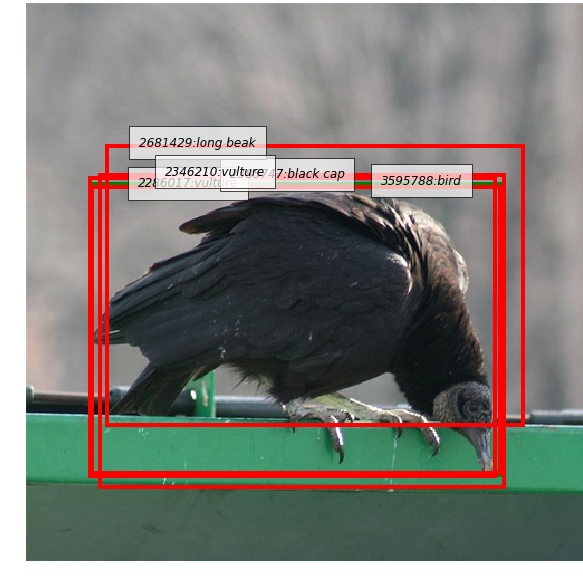
\includegraphics[scale=0.32]{figures/vulture.png} 
\begin{tabular}{lp{6cm}}
object id & linked region descriptions\\
\hline
3595788 & the \textbf{bird} is black in color, nose of the \textbf{bird}, a \textbf{bird} relaxing in stand, small white beak of \textbf{bird}, large black talon of \textbf{bird}, a \textbf{bird} on a green pole, a green bar under \textbf{bird}, black \textbf{bird} on green rail, small black eye of \textbf{bird}\\
2286017 & large black \textbf{vulture} on fence, a vulture on bar\\
%2385747 & small white beak of \textbf{bird}\\
2681429 & a semi \textbf{long beak}\\  
2346210 & a black and gray \textbf{vulture}\\
 \end{tabular}
\caption{Bounding boxes, names and region descriptions for an object in VisualGenome}
\label{fig:bird}
\end{center}
\end{figure}

%%% Local Variables:
%%% mode: latex
%%% TeX-master: "lrec2020naming"
%%% End:
